\chapter[Experimental setup]{Experimental setup}
\label{chap:setup}

The high-gradient tests at CERN are carried out in the three X-band\footnote{The X-band is a segment of the electromagnetic spectrum in the region of the microwaves. The waves in this region have frequencies between 8.0 and 12.0 GHz.} test stands (XBOXs). These are setups able to provide the necessary high-power RF pulses to the structures under test. For the tests described in this work the presence of the beam inside the accelerating cavity is also necessary, and is provided by the electron linac of the CTF3. 


\section[Linac and dogleg]{Linac and Dogleg}

As mentioned in the first chapter, the main goal of the CTF3 is to demonstrate the feasibility of the CLIC acceleration scheme. For this reason, the linac is used to generate the Drive Beam pulse, that is sent to the rings for the recombination and then to the prototype Two-beam module. 

The linac is realised using conventional 3 GHz technology. The recombination process leads to the bunch frequency of 12 GHz. 

Given that the breakdown rate tests of high-gradient cavities was not in the initial design of the facility and differs from the standard operation, in the following sections only the part of the setup which is relevant for the breakdown experiments will be described. The full CTF3 accelerator complex is widely described elsewhere \cite{CLIC:cdr,CTF:drive_beam,ctf3:dr}. 

To perform high-gradient structure tests, a beam line parallel to the linac has been used. The two beam lines are connected by an oblique segment, resulting in the characteristic shape that is the origin of the name \textit{Dogleg}.

For the high-gradient testing purpose the accelerator  simulates the CLIC Main Beam. The parameters of the beam are reported in the Table~\ref{beam_par_dogleg}


\begin{table}
  \centering
    \begin{tabular}{ c l }
    \toprule
    Current 		&	$1.6$ A\\
    Pulse length		&	$250$ ns\\
    Energy			&	$130$ MeV\\
    Reptition freq.	&	$0.83-25$ Hz\\
    \bottomrule
    \end{tabular}
\caption{Beam parameters used in the Dogleg \cite{NavarroQuirante:2025954}}
\label{beam_par_dogleg}
\end{table}



\subsubsection{Injector}

The production of the beam is realised by a 140-kV thermoionic gun, designed to deliver up to $5\,A$ of current in nominal operation conditions.
The gun is followed by a S-band\footnote{The S-band is the segment of the electromagnetic spectrum in the region of the microwaves. The waves in this region have frequencies between 2.0 and 4.0 GHz.} prebuncher and a 17 cell travelling-wave buncher. These structures are followed by two 1.2-m long accelerating structures. The beam dimension in this initial phase is controlled by means of solenoids, up to the second accelerating structure \cite{ctf:injector}.

Downstream of the injector a magnetic chicane with collimators is installed to eliminate off-energy particles and to perform bunch compression  \cite{Braun:999488}.

The layout of injector and chicane are reported in Fig.~\ref{injlayout}.

\subsubsection{Linac}

Three modules composed of two S-band accelerating structures operating at 3 GHz are installed in the linac. The accelerating structures consist of 32 regular cells, operating in the $2\pi/3$ mode. The damping of HOMs is guaranteed by radial slots in the iris, containing SiC loads. The structures are designed for fully loaded operation with a current of more than 4 A, but when simulating the Main Beam the current is significantly less, implying less loading. In this condition the energy gain is essentially bigger compared to Drive Beam operation.

The focusing is realised by triplets of quadrupoles, coupled with dipole correctors. The beam energy can be measured in the spectrometers in sector 4 and 10.

The layout of the linac is reported in Fig.~\ref{linaclayout}.

\subsubsection{The dogleg}

After sector 7 in the linac, another triplet of quadrupoles is located on the beamline, before a bending magnet. When the bending magnet is on, the beam is directed in the dogleg, passing through an oblique section, and is bent again to enter a segment of the beamline parallel to the linac. The optics of the dogleg beamline is designed to correct the dispersion provoked by the bending magnets \cite{Tecker:2013eba}. The structure under test is placed at the end of the dogleg line between two Beam Position Monitors (BPMs). Just before the structure there is a slit, in order to protect the coupling cell of the structure from being hit by a missteered beam. The beam is dumped downstream of the structure.

In case the first bending magnet is off, the beam proceeds straight in the linac, passing through a triplet of quadrupoles in section 9 and another triplet in sector 10. A spectrometer is placed after that, to measure the beam energy. 

The layout of the dogleg and of the linac up to section 10 is reported in Fig.~\ref{dolaut}.


\begin{landscape}
\begin{center}

\begin{figure}
\centering 
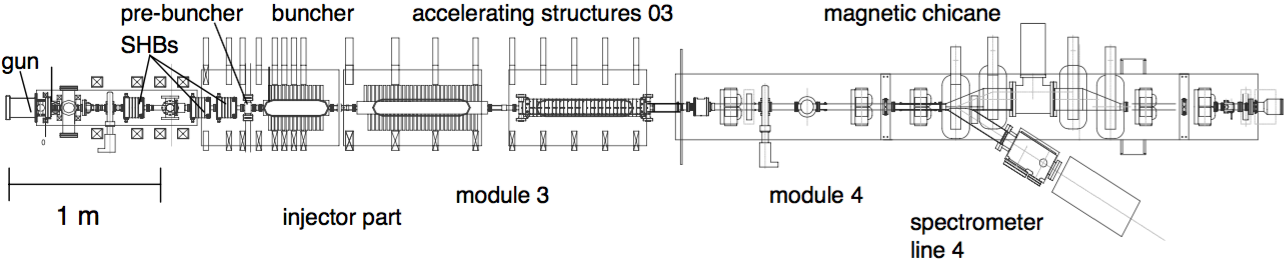
\includegraphics[width=23cm,keepaspectratio]{pictures/Injector}
\caption{Layout of the injector and the magnetic chicane. Legenda: SHBs: sub-harmonic bunchers.\vspace{4mm}}
\label{injlayout}
\end{figure}



\begin{figure}
\centering 
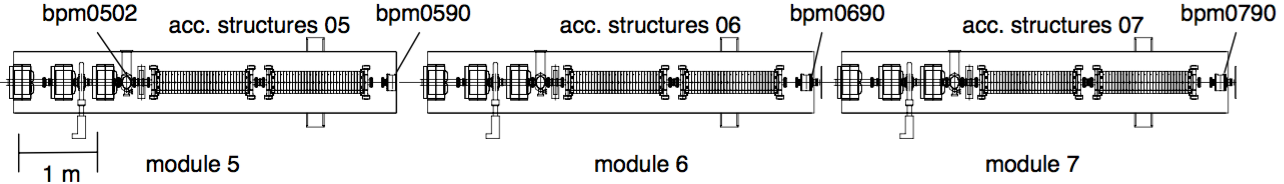
\includegraphics[width=23cm,keepaspectratio]{pictures/girder5-7}
\caption{Layout of the linac up to module 7. Legenda: bpm: beam position monitor.}
\label{linaclayout}
\end{figure}

\end{center}
\end{landscape}



\begin{landscape}
\begin{figure}
\centering 
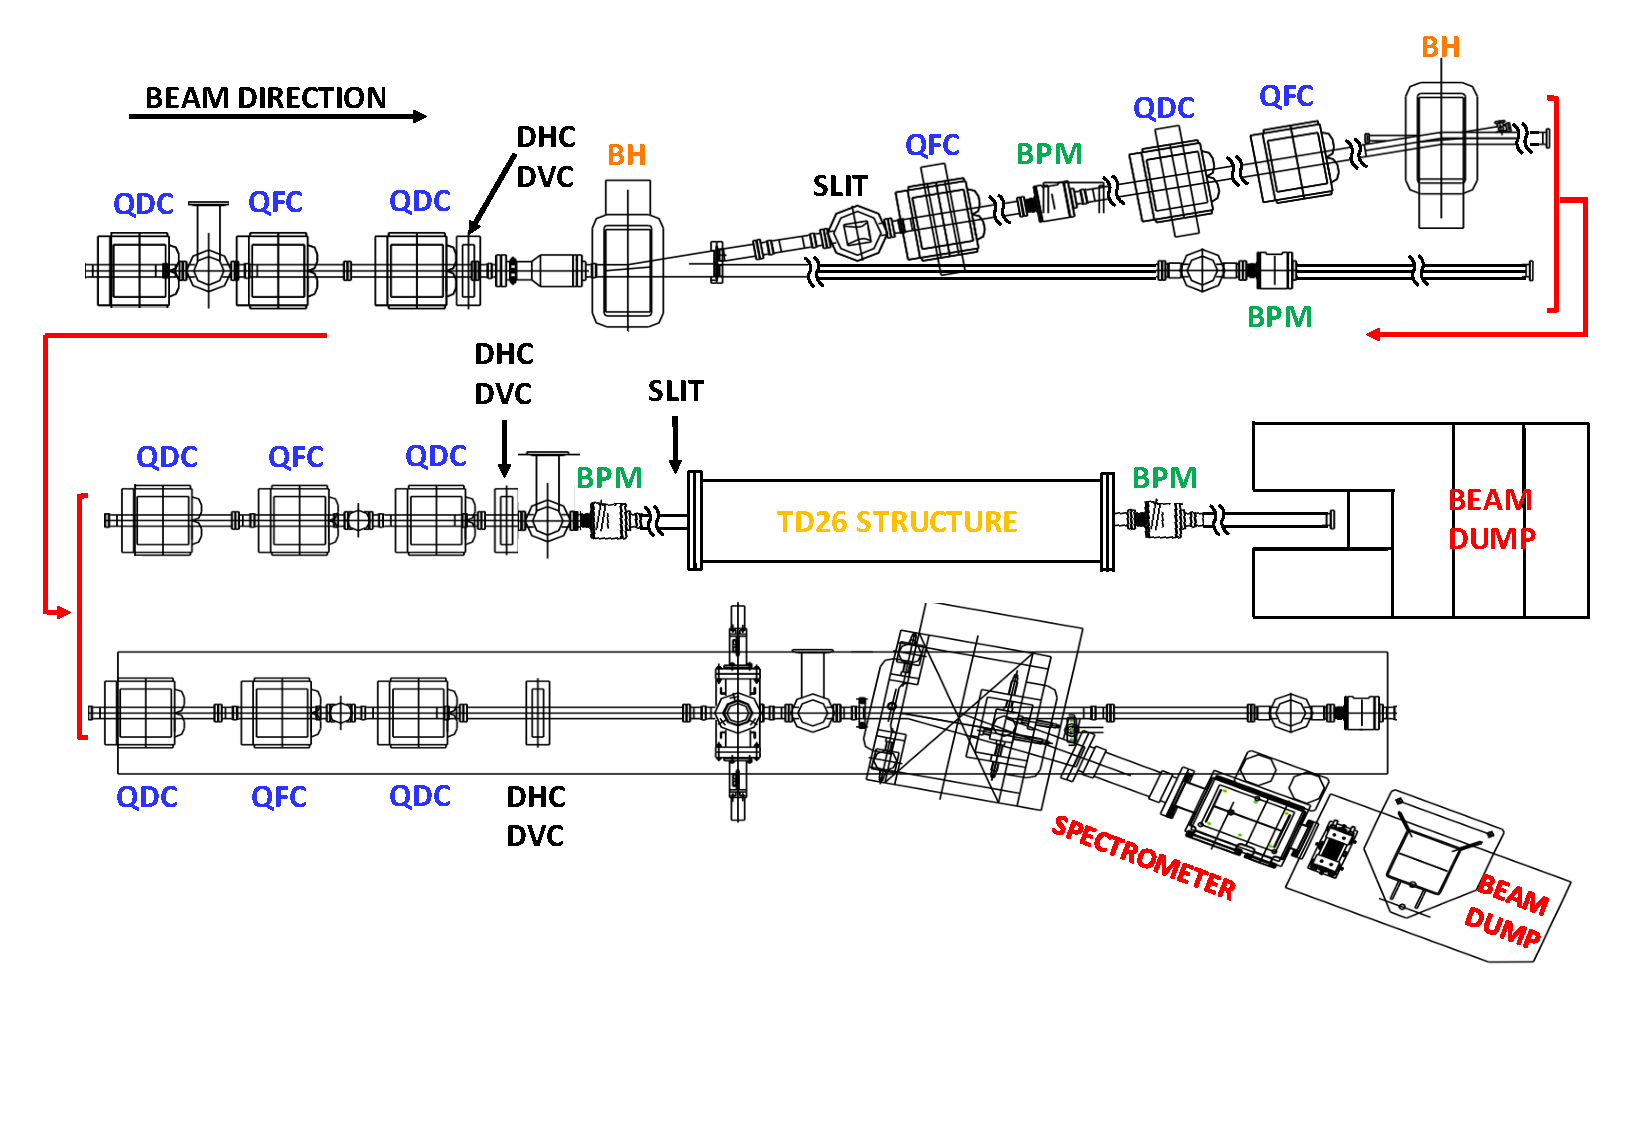
\includegraphics[scale=0.78]{pictures/modified_pets.pdf}
\caption{Simplified layout of optics and beam instrumentation of the dogleg line, adapted from technical drawings and facility layout \cite{EDMS:CTF3}. The beam for this section come from the end of the module 7. Legenda: QFC(QDC): focusing(defocusing) quadrupole; DHC(DVC): horizontal(vertical) dipole corrector; BH: bending magnet in horizontal plane; BPM: beam position monitor}
\label{dolaut}
\end{figure}
\end{landscape}



\section[RF power production]{RF power production}

The development of the accelerating cavity technology is strongly related to the possibility to produce and test prototypes. This test activity allows one to improve the understanding of the scaling laws of the phenomena that limit the performance of the accelerating structures, but also to compare the results of different production and conditioning techniques. 

At CERN the production of 12 GHz RF was once carried out only in the Two-beam modules in the CTF3. To enlarge the test capabilities standalone test stands were necessary. This was realised for the first time with the installation of the so called X-Band Test Stand 1 (XBOX1) \cite{Peauger:1287901}. Similar test stands are present in the Nextef facility at KEK and in the ASTA facility at SLAC. Currently there are three X-band test stands simultaneously active at CERN.

\begin{figure}[h]
\centering 
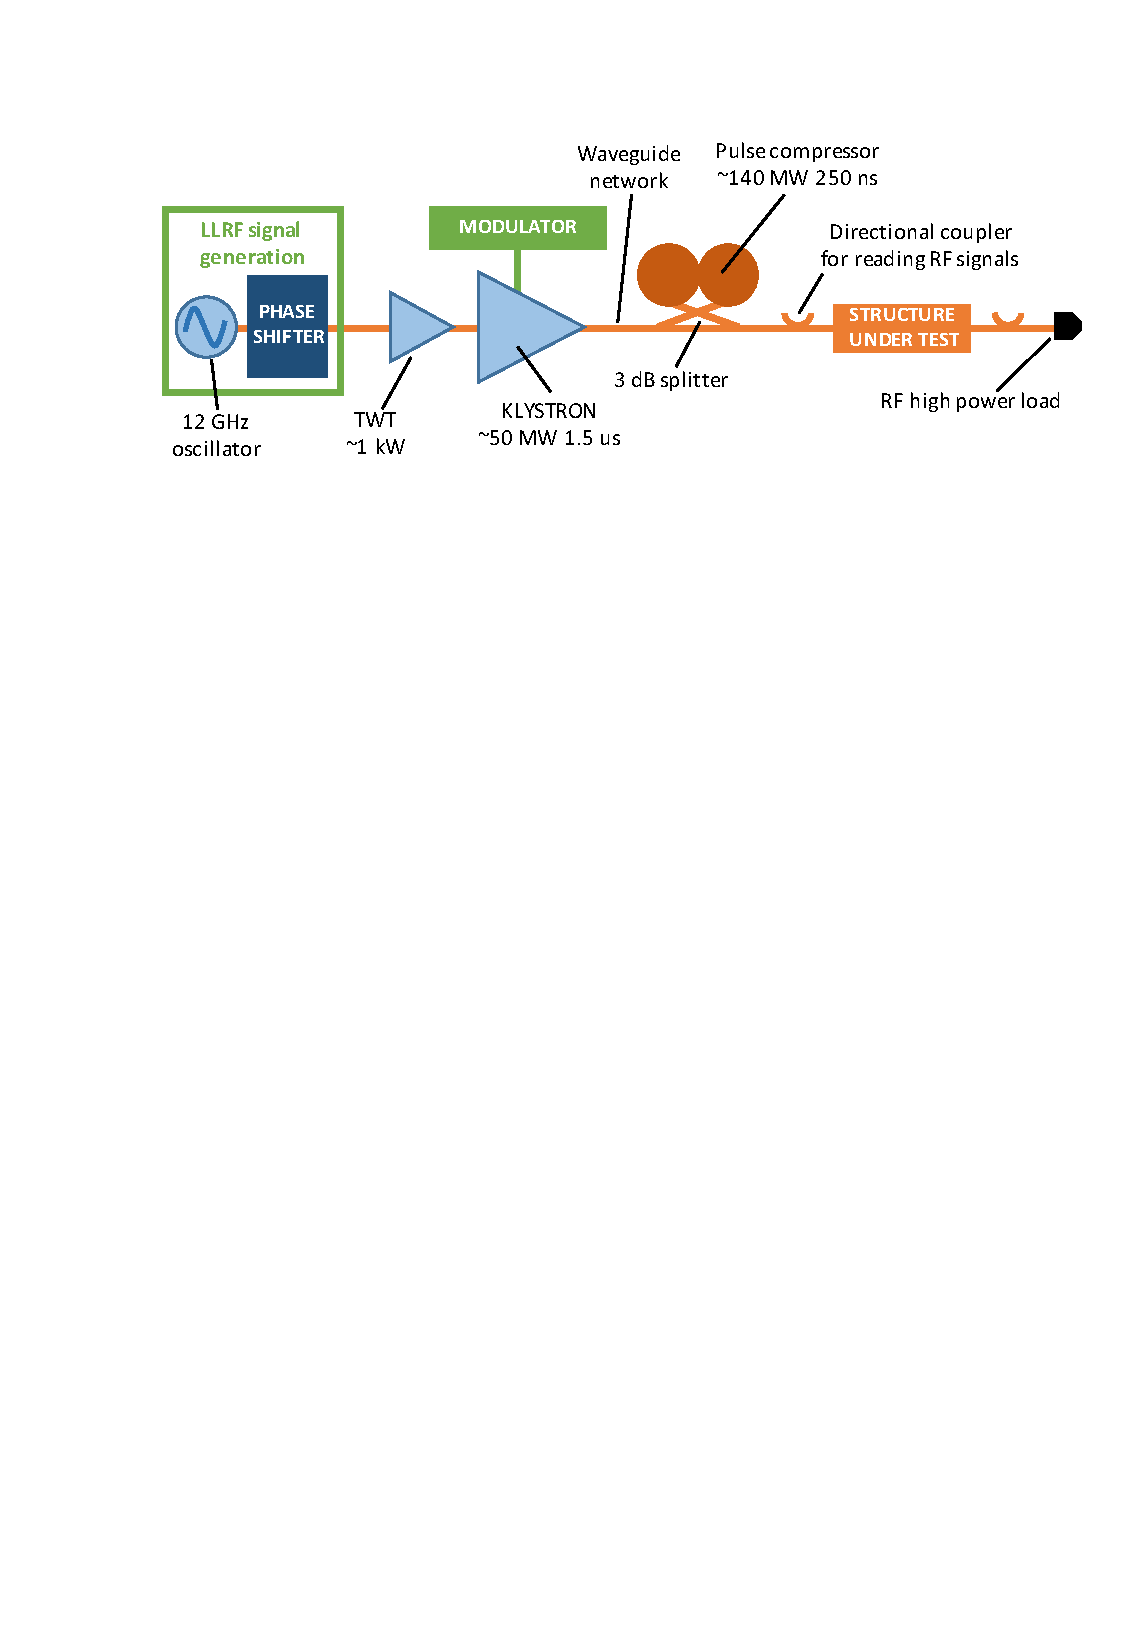
\includegraphics[scale=0.8]{pictures/test_stand_scheme.pdf}
\caption{Standalone X-band test stand layout}
\label{xbox_layout}
\end{figure}

The layout of a RF test stand is shown in Fig.~\ref{xbox_layout}. It is normally formed by signal generation, amplification and delivery systems; diagnostic and control systems, and service systems such as cooling and protection systems. 


\subsection[The X-Box1 at CERN]{The X-Box1 at CERN}

The proposal of an X-band test stand at CERN followed the change of the frequency of CLIC from 30 GHz to the european X-band 12 GHz in 2008. An organic description of XBOX1 is in \cite{Woolley:2015,Kovermann:1459879}. The high-power RF production is realised using:
\begin{itemize}
\item an XL-5 klystron, able to produce 50 MW of 12 GHz radiation with a pulse length of $1.5\, \mu$s and a repetition rate up to 50 Hz.
\item a Scandinova modulator, used to power the klystron.
\item a SLED-I type RF pulse compressor, able to compress the klystron output pulse to a shorter one of 140 MW, 250 ns long, which is sufficient to test accelerating structures considering the waveguide losses.
\end{itemize}

The RF delivery from the pulse compressor to the structure is realised using WR90 waveguides, kept under high-vacuum at a pressure of the order of\\ $5\times10^{-9}$ mbar. In order to reduce the losses, some part of the line to the structure under test is realised with low-loss waveguides. This structure requires mode converters because the fundamental modes of the waveguides are different. The overall transmission of the waveguide network has been measured to be around 67 \%.

More details regarding the key components of the system are presented in the following sections. The system is controlled solely by the Low-Level Radio Frequency (LLRF), since the gain of the amplification chain is fixed. This feature requires a unique control system of the LLRF together with the Data Acquisition system (DAQ), that will be described in section \ref{sec:RF_and_DAQ_s}.


\subsubsection{TWT, Klystron and modulator}

The very first power amplification stage is carried out by a Travelling Wave Tube (TWT) \cite{appSys:twt}, which is a device with the same working principle of the klystron (described below). It raises the power of the signal from some watts to up to 3 kW.

XL-5 klystrons comes from the effort made in SLAC to develop high efficiency klystrons for the Next Linear Collider project (NLC). They are based on the XL-4 klystrons, adapted from the american X-band frequency of 11.4~GHz to the european 12~GHz. This effort lead to the CPI VKX-8311A tubes that are currently in use \cite{klystron:CPI}, which are able to produce a pulse of 50 MW of power, $1.5 \, \mu$s long with an efficiency of the order of 40\%.
 
Klystrons are vacuum tube amplifiers. They are composed of a thermoionic gun, that emits a pulsed beam of electrons. The beam passes through one or several cavities, where a low power RF modulates the beam. After a drift space, where the beam is kept collimated by a solenoid and accelerated by a fixed DC field, the beam passes through a passive cavity that extracts the high power RF. The beam is then dumped. 

The klystron is operated in pulsed mode to reduce the wall-plug power consumption. This means that a power supply able to deliver short pulses of high power is necessary. XBOX1 uses a K-3 solid state modulator by Scandinova, able to supply voltage pulses up to 410 kV with currents of the order of 310~A.


\subsubsection{Pulse compressor}

The pulse compressor is the device used to convert the long pulse of the klystron into a shorter one at a higher power. The operation principle is that the power from the klystron is stored in high-Q resonant cavities during the pulse. Before the end of the pulse the cavities are emptied by reverting the phase of the input power. The emptying process is done in a shorter time than the filling time, determining the production of a short high power pulse. 

This technique can lead to peak power increase up to a factor 5-7. 

The SLED-I type pulse compressor is using two cavities, coupled with a 3~dB hybrid coupler, in order to discharge the produced power to the desired load instead of sending it back to the klystron. The theory behind the pulse compression is fully described in \cite{Fiebig:209756}, the application in XBOX1 in \cite{SLED:ctf3}.

The resonance frequency of the pulse compressor's cavities is strongly dependent on the volume, which depends on the temperature. For this reason the heat produced by the RF, due to the ohmic resistance of the walls, has to be disposed of by an external thermostatic system. An imperfect heat dissipation leads to the detuning of the cavities, which constitute an operational issue and will be extensively discussed later in section \ref{sec:xboxop} and \ref{sec:PCtune}.

 


\section[DAQ \& RF control systems]{DAQ \& RF control systems}
\label{sec:RF_and_DAQ_s}

The control system is in charge of generating a phase-modulated signal for the successive amplification stages (TWT and klystron). It also has to acquire the signals from the directional couplers, and the diagnostic signals from the structure and the vacuum systems. According to the diagnostic inputs, it modulates the signal and can also act on the beam permit of the gun of the linac. This last role is central, since the interlocking function is fundamental not only for the equipment protection, but also to trigger the data memorisation. 


\subsection[Hardware]{Hardware}

To perform his task, the control system is made of different components, including PLCs (Programmable Logic Controller) interlock systems,  VME (Versa Module Europa) crate based arbitrary signal generators, OASIS PC \cite{OASIS}-based digitisers and PXI (PCI eXtension Instrumentation)-based control systems.

The core of the system is the National Instrument PXI crate \cite{NI:PXI}, that is the most advanced system in the setup. It carries out the acquisition and processing of all the signals relevant for interlocking the system; triggers the interlocks; save in the internal memory the recorded signals and retrieves the signals sampled externally in case of an interesting event; interfaces with the rest of the instrumentation.

Since the phase of the LLRF signal has to be modulated to be able to perform the pulse compression, the LLRF signal is sent to an analog and a digital phase shifter in series. During the experiments with beam, the digital one is used to properly phase the RF with respect to the beam.

The data acquisition from the -50 dB directional couplers on the waveguides is performed using different kind of sensors:
\begin{enumerate}
\item Diodes with a bandwidth of 500MHz convert the RF signals to a DC voltage level
\item IQ\footnote{In-phase and quadrature components demodulators. These detectors measure amplitude and phase of an electromagnetic wave by mixing it to a known wave at the same frequency (in this case supplied by the main 12 GHz oscillator of the Xbox).} demodulators are used to measure the phase and the amplitude
\item Logarithmic detectors are used to acquire the signals with a wide dynamic range of over 46 dB
\end{enumerate}

The PXI crate has 8 channels of 14-bits, 250 MSa/s digitisers. These digitisers are connected internally to FPGAs in order perform the analysis as fast as possible, and send a signal to the trigger unit to interlock the LLRF signal production. A 24 channel Digital Multimeter (DMM) unit is used to read the vacuum signals from the ion pump controllers. The fast digitisers of the PXI acquire the signals from the logarithmic detectors. 

The signals of the IQ demodulators are sampled by OASIS acquisition PC containing 16 units of 1 GSa/s, 8-bits ADCs. These are read by the PXI crate for the breakdown events and archived for the offline analysis. 

The signals of the BPMs are acquired and recorded as well by one of the acquisition cards of the PXI crate.

Figure \ref{high_l_RF} shows schematically the high level RF described above and the acquisition equipment that is used for diagnostic and data analysis.

\begin{figure}[h]
\centering 
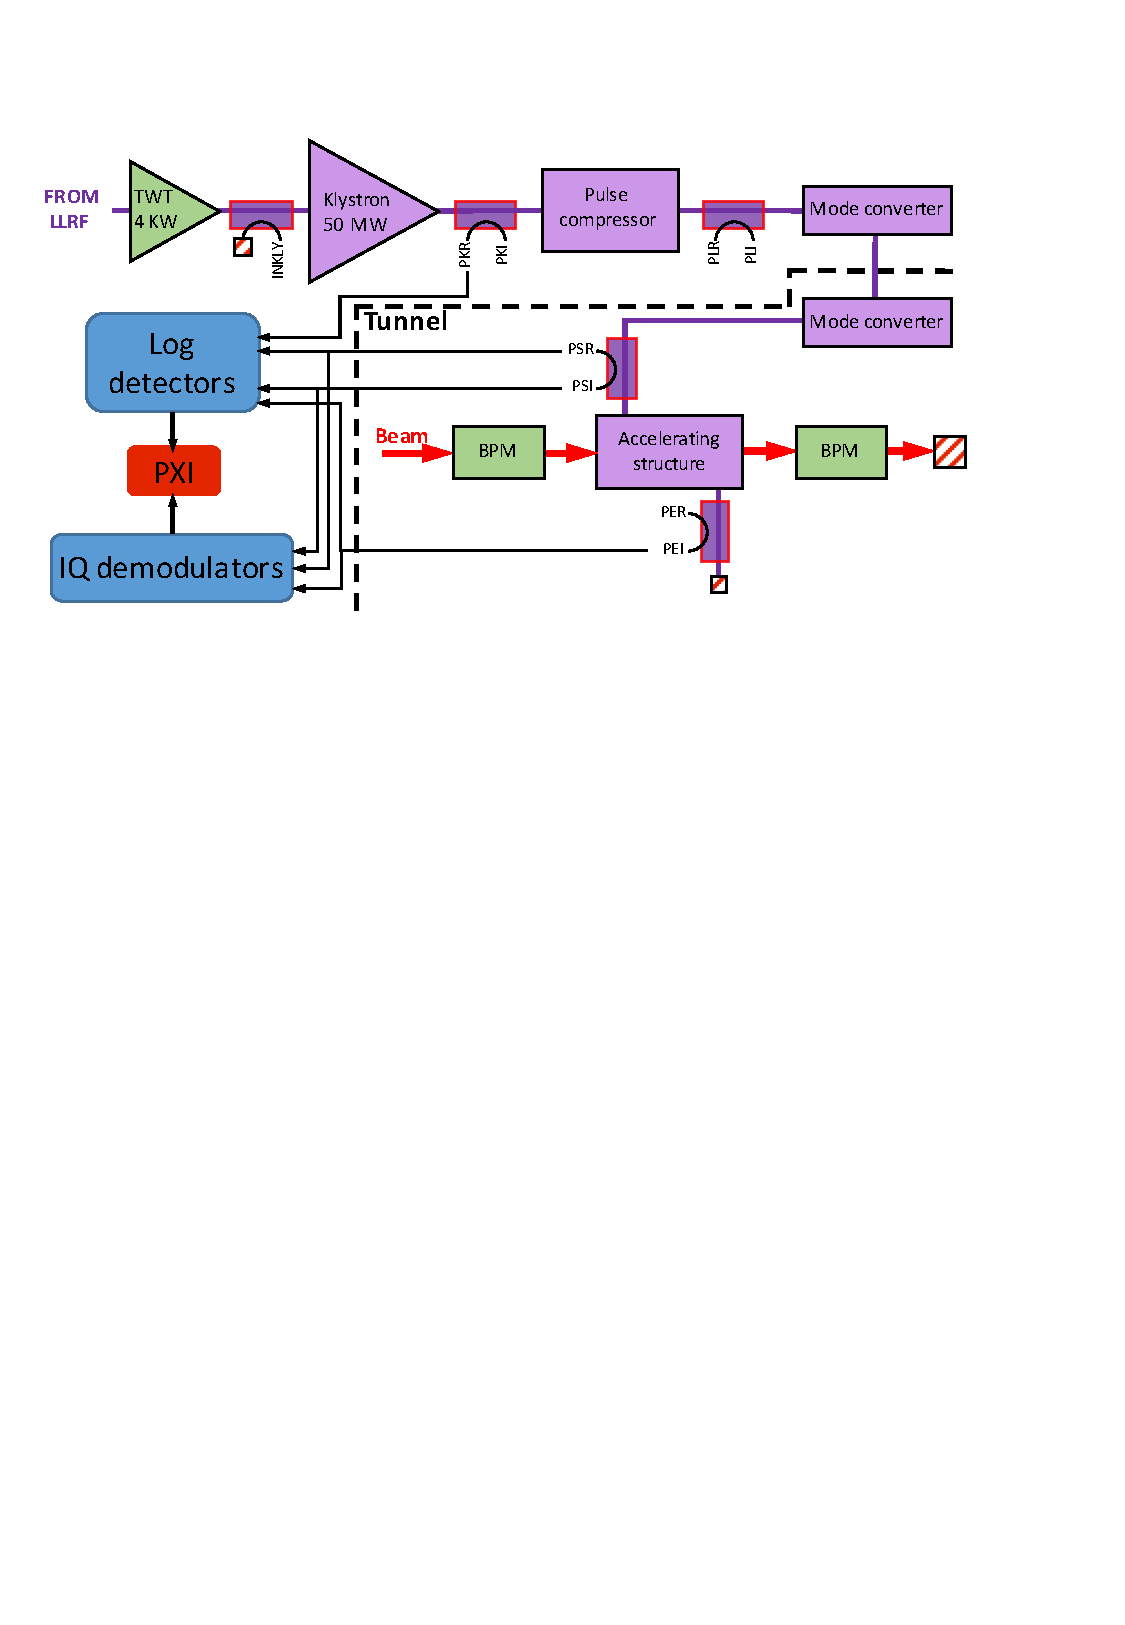
\includegraphics[scale=0.8]{pictures/high-level-RF-scheme.pdf}
\caption{Schematic of the high level RF and the relevant part of the DAQ for the interlock system. See appendix for glossary of abbreviations}
\label{high_l_RF}
\end{figure}



\subsection[Online triggers]{Online triggers}
 \label{subs:itlk}

An interlocking system is implemented in the PXI crate, in order to detect the breakdown events and trigger the data saving. When one of the interlocks is triggered, it acts on the LLRF power, cutting the power but leaving the rest of the amplification chain ready. After a period of time, generally seconds, the power is restarted and ramped up gradually.

There are four interlocks of this kind, triggered when one of the following quantities exceedes a user-defined threshold:
\begin{enumerate}
\item {\makebox[7cm]{Cavity peak reflected power:\hfill} $max(P_{REF})$}
\item {\makebox[7cm]{Cavity reflected energy:\hfill} $\int P_{REF}(t) \, dt $}
\item {\makebox[7cm]{Cavity missing transmitted energy:\hfill} $\int P_{INC}(t)\,dt - \int P_{TRA}(t)\,dt$}
\item {\makebox[7cm]{Peak power reflected to the klystron:\hfill} $max(P_{KREF})$}
\end{enumerate}
The purpose of the last interlock is protect the klystron, and is triggered when the reflected power back from the pulse compressor is too high. This happens especially when the pulse compressor is not properly tuned, as described later in this chapter.
The first three indeed are used to detect a breakdown event inside the structure under test. When one or more of these four interlock is triggered, the event is saved by the PXI crate. In addition, an event is saved every minute, to monitor the state of the current test.

Generally a breakdown event triggers more than one of the criteria above. A key point is the redundancy: any of the interlocks triggers the event recording in order to not to lose any interesting event. Additional events that trigger the saving are stored anyway, and will be filtered out during the offline analysis described in the next chapter.


\section[Other systems]{Other systems}

\subsubsection{Cooling system}

The operation of CLIC requires a component alignment on the $\mu$m scale. Once realised during the installation, the alignment has to be maintained keeping the thermal dilation under control. A number of studies have been carried out to this purpose, such as \cite{Daskalaki:2141828}. The thermal data from the accelerating structure installed in the dogleg are currently analysed as part of these studies.

The heating of the accelerating structures is provoked by the Joule heating induced by the RF encountering the resistive walls. In nominal conditions the heating is constant once the structure is running at constant RF input power. 

In this perspective the breakdown events have a key role since they modify the heating, because of the perturbation of the RF power flow. This materialises both because of the power reflection by the plasma in the accelerating cavity, and the huge amount of power absorbed by the plasma, that can achieve the level of tens of MW.


\subsubsection{Vacuum system}

In every accelerator an adequate vacuum has to be reached to preserve the quality of the beam. Compared to the traditional vacuum systems, in accelerators there are additional phenomena taking place. In fact, in addition to permeation, the desorbtion of surfaces is enhanced by beam losses and the photon emission from the beam. 

An adequate pumping system is hence necessary, and is described in \cite{ctf3:dr}.

On top of the vacuum system for the beam pipes, the waveguide network has to be kept under high vacuum. Also in this case there is an additional effect to the permeation, that is similar to the beam losses. The plasma that establishes during the breakdown process is formed by material evaporated from the cathode, and needs to be pumped out to restore the vacuum level as soon as possible. Furthermore, the vacuum arc emits electrons and ions that can enhance desorbtion.


\section[Operation of the setup]{Operation of the setup}

One of the main tasks of the author of the thesis was to carry out the operation and supervision of the accelerator and of the 12 GHz RF production, in addition to the data analysis. It seems therefore appropriate to spend some words on the operation and the operational issues encountered in the CTF3.

\subsection{Linac operation}

During 2016 the CTF3 schedule foresaw running the Drive Beam during the week and switching to the Main Beam for the weekend. The reason is that the high-gradient testing experiments require a long beam time to collect data, because of the low breakdown rates. So they are be carried out by leaving the accelerator running when it is not in use by other operators. A reliable system of interlocks is diagnosing the equipments and ensuring the protection of the accelerator. 

As mentioned before, the linac of the CTF3 is normally operated in fully-loaded mode, producing a long  high-current beam pulse of the Drive Beam. In order to produce the Main Beam for the BD tests, it is necessary to produce a short beam pulse with a lower current and a resulting higher energy. 

The accelerating structures in the linac are powered by 45 MW klystrons equipped with pulse compressor system. 
The RF pulse shape is changed by modifying the phase program of the low level RF.

The current pulse duration from the gun is also adapted to the new beam. The beam optics was calculated to minimise the beam size in the accelerating structure, and the quadrupole gradients are set up accordingly.

This operation required normally slightly less than an hour, mainly due to temperature settling of the RF pulse compressors, sometimes up to a couple of hours.

The operation has to be supervised during the running, since the trip of some component can cause an interruption of the beam or of the RF production. The operation has been automatised to restart after the most common trips without operator intervention. Nevertheless, other faults have to be dealt with manually. The typical uptime without intervention is around one day.

\subsection{Xbox operation}
\label{sec:xboxop}

The repetition rate used is 25 or 50 Hz, to accumulate higher statistics.

After a breakdown, the power is stopped as foreseen in the CLIC operational scenario. After the stop, the power is gradually ramped up. Overall, the power restoration lasts less than 10 s if no other breakdown happen.

Power dissipation changes leads to detuning of the pulse compressor. The detuning can be provoked by frequent breakdowns (which stops the RF production),  switching from loaded to unloaded condition (normally because of problems on the linac; the RF input power level is lowered in some cases when there is no beam), or from the thermal day-night excursion. The pulse compressor detuning is accompanied by the increase of reflections to the klystron. A tuning algorithm has been implemented to face this effect. More details about the tuning will be given in section \ref{sec:PCtune}.